\subsection{Cơ Sở Lý Thuyết}
% -----------------------------------------------------------------------------

Mô hình hồi quy bội tổng quát:
\[
  Y = \beta_0 + \beta_1 X_1 + \beta_2 X_2 + \cdots + \beta_p X_p + \varepsilon
\]

Giả định tuyến tính phát biểu rằng:
\[
  E[Y \mid X_1, X_2, \ldots, X_p] = \beta_0 + \beta_1 X_1 + \cdots + \beta_p X_p
\]

Hay nói cách khác: \textbf{kỳ vọng có điều kiện của $Y$ là một hàm tuyến tính trong các tham số $\beta$}
\cite[Sec.~7.3.1, p.~141]{rencher2008linear}.

\subsubsection{Ý nghĩa cốt lõi 1: Cấu trúc đại số của các tham số \texorpdfstring{$\beta$}{beta}}

``Tuyến tính'' ở đây là thuộc tính về \textbf{cấu trúc đại số của $\beta$}, không phải hình dáng của dữ liệu. Cụ thể, các tham số $\beta_0, \beta_1, \ldots, \beta_k$ phải:
\begin{itemize}
  \item Xuất hiện ở \textbf{bậc một} (không có $\beta^2$, $\beta^3$, \ldots)
  \item Đứng \textbf{độc lập}, không lồng trong hàm phi tuyến
  \item Được \textbf{cộng lại} với nhau để tạo thành dự báo
\end{itemize}

Bạn sẽ không bao giờ thấy dạng $\beta^2$, $e^{\beta}$, hay $\sin(\beta)$ trong một \textit{mô hình tuyến tính}.


\subsubsection{Ba nghĩa khác nhau của tuyến tính}

Trong hồi quy, cùng một từ tuyến tính có thể chỉ ba khái niệm khác nhau. Bảng sau tách riêng ba tầng này để tránh nhầm lẫn giữa định nghĩa mô hình, giả định về hàm trung bình, và hình dạng đồ thị quan sát được.

\begin{center}
\small
\begin{tabularx}{\textwidth}{@{}>{\raggedright\arraybackslash}p{3.5cm}>{\raggedright\arraybackslash}X>{\raggedright\arraybackslash}X@{}}
\toprule
\textbf{Khái niệm} & \textbf{Ý nghĩa} & \textbf{Vai trò trong hồi quy} \\
\midrule
Tuyến tính theo tham số & Các $\beta$ xuất hiện bậc một và cộng tính & Điều kiện để thuộc lớp mô hình tuyến tính \cite[Sec.~7.3.1, p.~141]{rencher2008linear} \\
Tuyến tính của $E(Y\mid X)$ & Hàm trung bình có điều kiện được chỉ định đúng theo các biến đang xét & Giả định về dạng sinh dữ liệu và mean function \cite[Sec.~1.2; Sec.~3.4.1]{weisberg2014applied} \\
Hình dạng đồ thị theo $X$ & Đường dự báo có thể thẳng hoặc cong trên trục biến ban đầu & Đa thức và splines có thể tạo đường cong nhưng vẫn tuyến tính theo $\beta$ \cite[Ch.~5, pp.~109--115]{weisberg2014applied} \\
\bottomrule
\end{tabularx}
\end{center}

\subsubsection{Ý nghĩa cốt lõi 2: Sự tự do của các biến \texorpdfstring{$x$}{x}}

Ngược lại, \textbf{mô hình không đặt bất kỳ ràng buộc nào lên các biến $x$}. Bạn hoàn toàn có thể biến đổi $x$ thành bất kỳ dạng phi tuyến nào (bình phương, nghịch đảo, logarit, hàm lượng giác, \ldots) và mô hình vẫn là \textit{mô hình tuyến tính}. Ví dụ, phương trình sau chứa đồng thời nghịch đảo ($x_2^{-1}$), bình phương ($x_2^2$) và hàm sin ($\sin x_2$):
\[
  y = \beta_0 + \beta_1 x_1 + \beta_2 x_2^{-1} + \beta_3 x_2^2 + \beta_4 \sin(x_2) + \varepsilon
\]

Mô hình này \textbf{vẫn là mô hình tuyến tính} vì $\beta_0, \ldots, \beta_4$ đều xuất hiện ở bậc một và được cộng lại.

\subsubsection{Vì sao phi tuyến theo \texorpdfstring{$X$}{X} được phép, nhưng phi tuyến theo \texorpdfstring{$\beta$}{beta} thì không?}

Điểm mấu chốt nằm ở vai trò khác nhau của hai đại lượng. Các biến $X$ là dữ liệu đã quan sát được; sau khi thu thập dữ liệu, $x$, $x^2$, $\log x$ hay $\sin x$ đều chỉ là những cột số liệu đã biết trong ma trận thiết kế. Ngược lại, $\beta$ là tham số chưa biết cần ước lượng. Vì vậy, một mô hình được gọi là tuyến tính không phải vì đồ thị $Y$ theo $X$ nhất thiết là đường thẳng, mà vì kỳ vọng có điều kiện được viết dưới dạng \textbf{tổ hợp tuyến tính của các tham số chưa biết}.

Về mặt hình học, thêm $x^2$ không phá vỡ tính tuyến tính của mô hình. Nó chỉ mở rộng không gian dự báo bằng một trục mới. Chẳng hạn, $Y = \beta_0 + \beta_1 x + \beta_2 x^2 + \varepsilon$ tạo ra một đường parabol nếu vẽ theo trục $x$ ban đầu, nhưng trong không gian có các trục $1$, $x$ và $x^2$, phần dự báo vẫn nằm trên một siêu phẳng tuyến tính do các cột của ma trận thiết kế sinh ra.

Lý do quan trọng nhất là khả năng ước lượng. Khi mô hình tuyến tính trong $\beta$, bài toán OLS
\[
  \min_{\boldsymbol{\beta}} \|\mathbf{y} - \mathbf{X}\boldsymbol{\beta}\|^2
\]
dẫn đến hệ phương trình chuẩn tuyến tính và nghiệm dạng đóng. Nếu tham số xuất hiện phi tuyến, ví dụ $Y = \beta_0 + \beta_1 e^{\beta_2 x} + \varepsilon$ hoặc $Y = \theta_1 + \theta_2(1 - e^{-\theta_3 x}) + \varepsilon$, đạo hàm của tổng bình phương phần dư không còn tạo ra một hệ tuyến tính đơn giản. Khi đó ta phải dùng các thuật toán lặp như Gauss--Newton, cần giá trị khởi đầu và có rủi ro không hội tụ hoặc hội tụ về cực tiểu cục bộ.

\vspace{6pt}
\begin{center}
\small
\begin{tabularx}{\textwidth}{@{}>{\raggedright\arraybackslash}Xc>{\raggedright\arraybackslash}X@{}}
\toprule
\textbf{Dạng mô hình} & \textbf{Tuyến tính trong $\beta$?} & \textbf{Lý do} \\
\midrule
$Y = \beta_0 + \beta_1 X + \varepsilon$ & Có & $\beta$ bậc một, cộng tính \\
$Y = \beta_0 + \beta_1 X + \beta_2 X^2 + \varepsilon$ & Có & $X^2$ là biến mới; $\beta$ vẫn bậc một \\
$Y = \beta_0 + \beta_1 \log X + \beta_2 X^{-1} + \varepsilon$ & Có & $\log X,\; X^{-1}$ là biến mới \\
$Y = \beta_0 \cdot e^{\beta_1 X} + \varepsilon$ & \textbf{Không} & $\beta_1$ nằm trong $\exp(\cdot)$ \\
$Y = \beta_0 + X^{\beta_1} + \varepsilon$ & \textbf{Không} & $\beta_1$ là số mũ của $X$ \\
\bottomrule
\end{tabularx}
\end{center}

\textbf{Hệ quả thực tiễn.} Nhờ đặc tính này, khuôn khổ hồi quy tuyến tính có thể xấp xỉ vô số quan hệ cong trong thực tế, chỉ bằng cách biến đổi các biến $x$, trong khi vẫn giữ nguyên phương pháp tính toán OLS.

\textbf{Minh họa hình học: ba trường hợp đặc trưng.}

\begin{figure}[H]
  \centering
  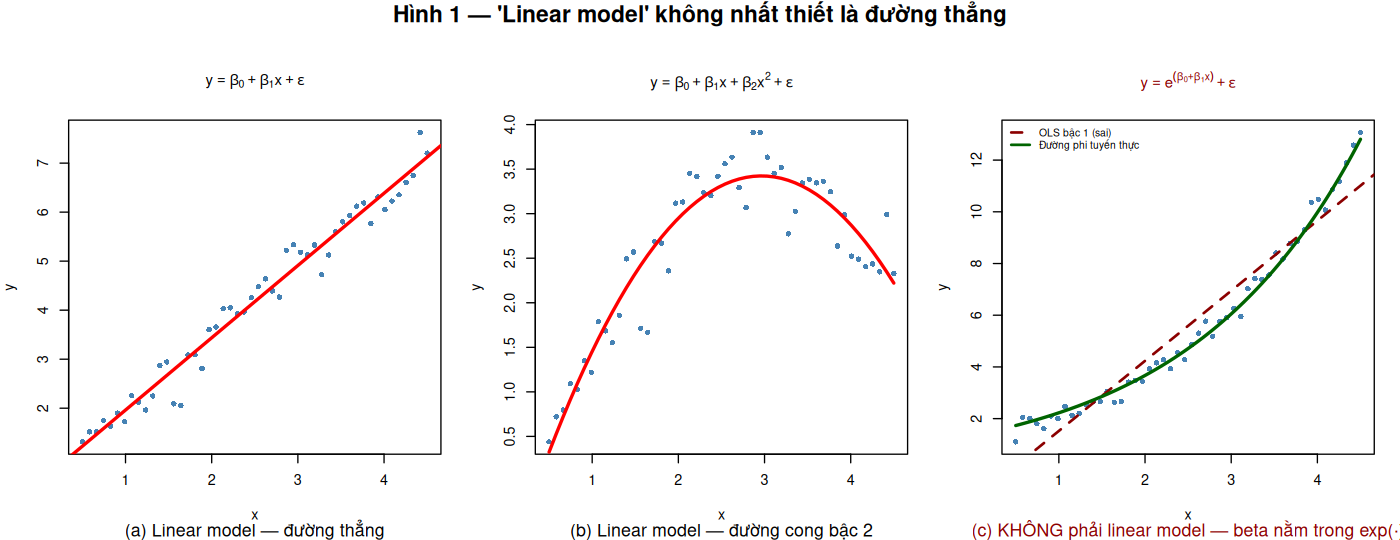
\includegraphics[width=\textwidth]{./figures/fig1_linear_params.png}
  \caption[Mô hình tuyến tính không nhất thiết tạo ra đường thẳng]{Mô hình tuyến tính không nhất thiết tạo ra đường thẳng.
  \textbf{(a)} Bậc 1 $\to$ đường thẳng.
  \textbf{(b)} Bậc 2 $\to$ parabol, vẫn là mô hình tuyến tính vì $\beta_0, \beta_1, \beta_2$ bậc một.
  \textbf{(c)} $y = e^{\beta_0+\beta_1 x}$: $\beta_1$ nằm trong $\exp(\cdot)$, không phải mô hình tuyến tính.}
  \label{fig:linear_params}
\end{figure}

\subsubsection{Dạng Ma Trận: Biểu Diễn Gọn Cho \texorpdfstring{$n$}{n} Quan Sát}

Với $n$ quan sát, dạng đại số tổng quát được gom lại thành phép nhân ma trận:
\[
  \mathbf{y} = \mathbf{X}\boldsymbol{\beta} + \boldsymbol{\varepsilon},
  \qquad
  E(\mathbf{Y} \mid \mathbf{X}) = \mathbf{X}\boldsymbol{\beta}
\]

trong đó:
\begin{itemize}
  \item $\mathbf{y}$: vector cột $n \times 1$ chứa các giá trị phản hồi.
  \item $\mathbf{X}$: \textbf{ma trận thiết kế} kích thước $n \times (k+1)$, cột đầu là vector đơn vị $\mathbf{1}_n$ (cho $\beta_0$), các cột còn lại là giá trị của $k$ biến dự báo.
  \item $\boldsymbol{\beta} = (\beta_0, \beta_1, \ldots, \beta_k)^\top$: vector cột $(k+1) \times 1$ chứa các tham số.
  \item $\boldsymbol{\varepsilon}$: vector cột $n \times 1$ chứa các sai số ngẫu nhiên.
\end{itemize}

Nhờ cấu trúc tổ hợp tuyến tính này, OLS tối thiểu hóa $\|\mathbf{y} - \mathbf{X}\boldsymbol{\beta}\|^2$ và dẫn đến \textbf{hệ phương trình chuẩn}:
\[
  \mathbf{X}^\top\mathbf{X}\,\hat{\boldsymbol{\beta}} = \mathbf{X}^\top\mathbf{y}
\]

Khi $\mathbf{X}^\top\mathbf{X}$ khả nghịch (các cột của $\mathbf{X}$ độc lập tuyến tính), nghiệm duy nhất là $\hat{\boldsymbol{\beta}} = (\mathbf{X}^\top\mathbf{X})^{-1}\mathbf{X}^\top\mathbf{y}$. Đây là lý do tính tuyến tính trong $\boldsymbol{\beta}$ mang lại phương pháp ước lượng \textbf{đồng nhất và khả tính} cho mọi cấu hình biến dự báo.

\subsubsection{Liên hệ với giả định \texorpdfstring{$E(\varepsilon \mid X) = 0$}{E(epsilon | X) = 0}}

Giả định tuyến tính và giả định $E(\varepsilon \mid X) = 0$ là \textbf{hai mặt của cùng một yêu cầu}: khi dạng hàm $E[Y|X]$ được chỉ định đúng, phần dư chỉ là nhiễu ngẫu nhiên, kỳ vọng của chúng bằng 0 tại mọi giá trị $X$. Khi dạng hàm sai, phần dư mang theo thông tin có hệ thống và $E(\varepsilon \mid X) \neq 0$.

\begin{figure}[H]
  \centering
  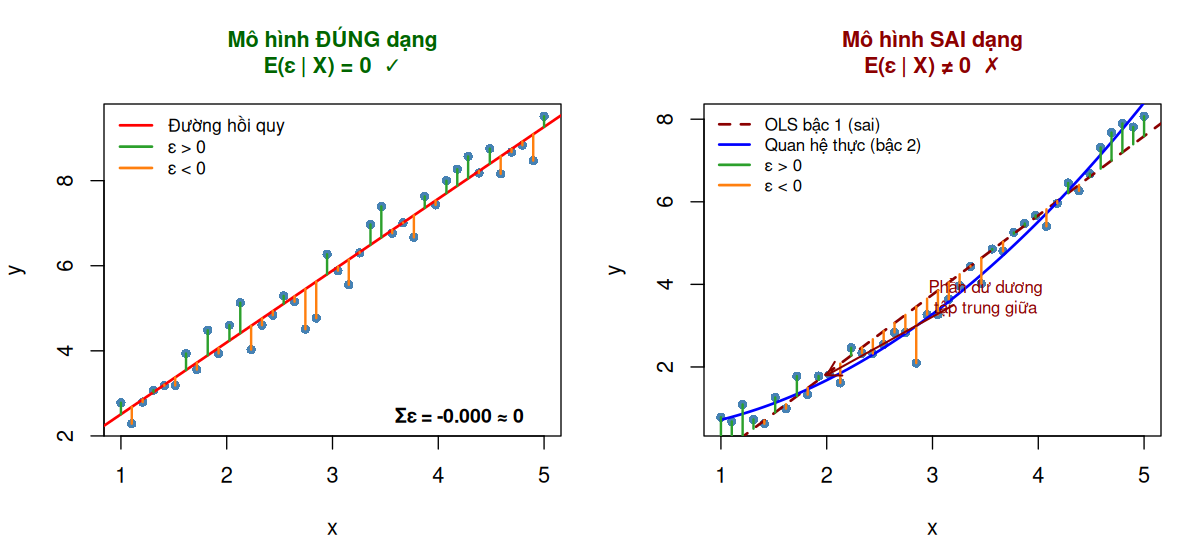
\includegraphics[width=0.9\textwidth]{./figures/fig2_epsilon_zero.png}
  \caption{$E(\varepsilon|X)=0$ khi mô hình đúng dạng (trái) vs.\ $E(\varepsilon|X)\neq 0$ khi sai dạng (phải).
  Trái: phần dư dương (xanh) và âm (cam) phân bố đều hai phía, $\sum\varepsilon\approx 0$.
  Phải: phần dư dương tập trung ở giữa, âm ở hai đầu, tạo thành mẫu hình có hệ thống.}
  \label{fig:epsilon_zero}
\end{figure}

% -----------------------------------------------------------------------------
